\begin{figure*}[t]
    \centering
    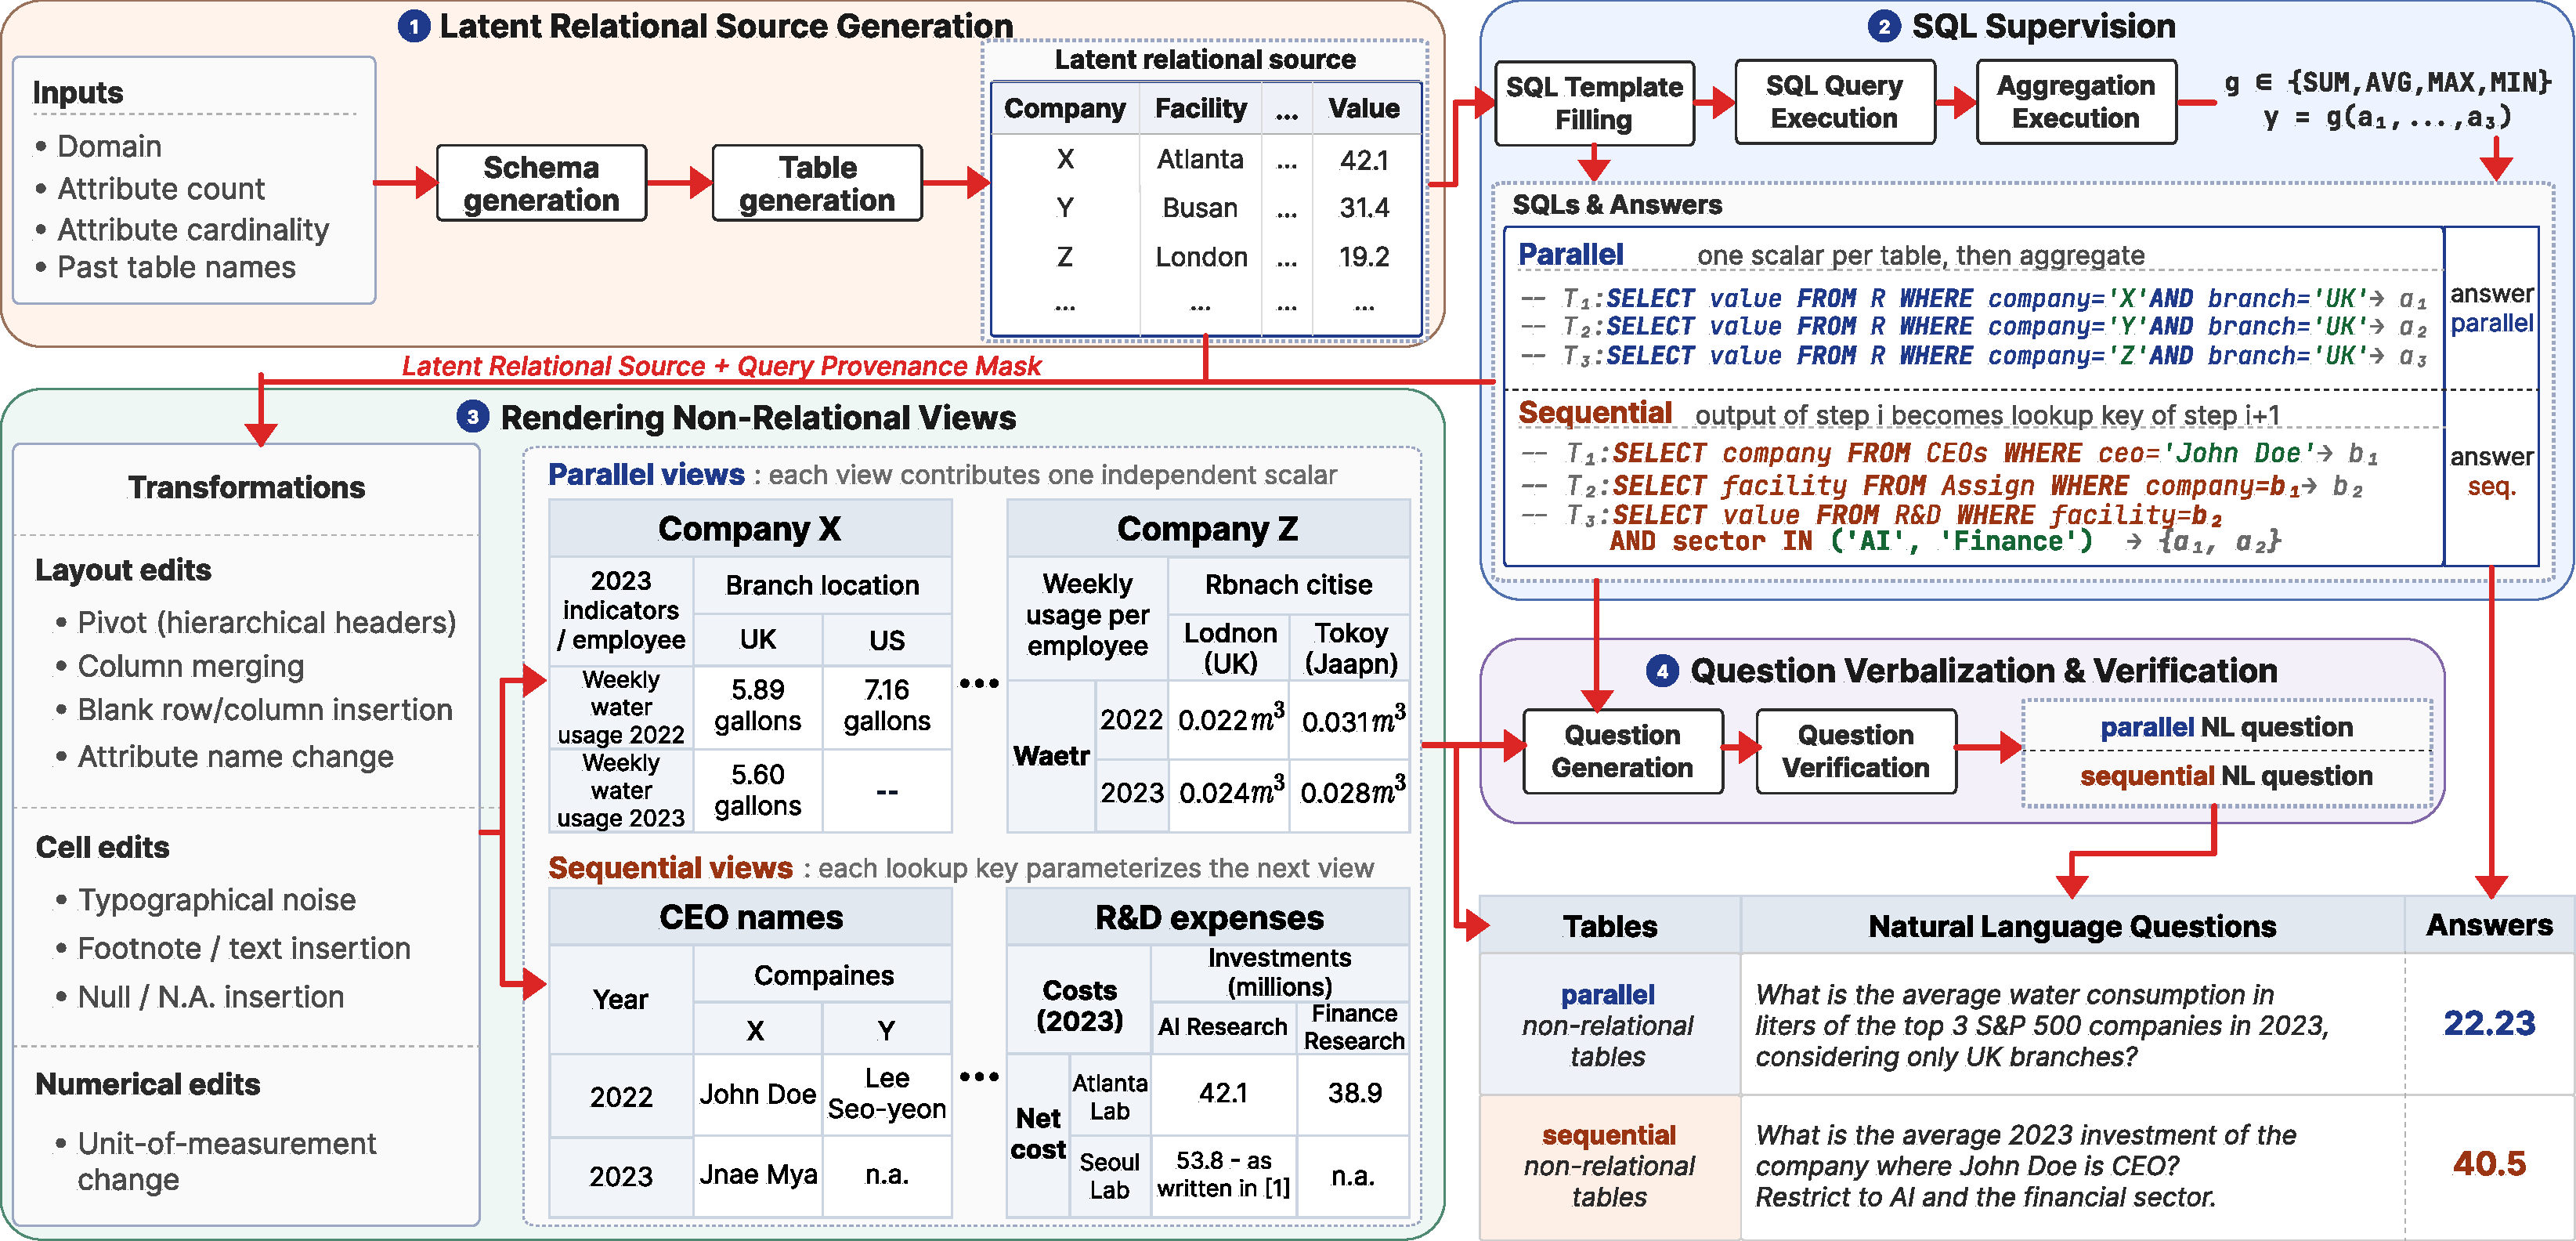
\includegraphics[width=\linewidth]{img/gradino.pdf}
    \caption{Overview of \name. A latent relational source provides SQL supervision and gold answers, while models are evaluated only on perturbed non-relational views.}
    \label{fig:pipeline}
    \vspace{-6pt}
\end{figure*}

\section{Related Work} 
\label{sec:rw}
\noindent{\bf Table QA benchmarks and robustness to tabular perturbations.}
Early Table QA benchmarks focused on relational tables, from single-table semantic parsing~\cite{1.4} to multi-table relational QA~\cite{1.6,1.19,1.20,1.30}, but these resources are largely limited to contrived relational schemas and textbook-style joins that do not reflect the presentation and layout irregularities common in real documents. Subsequent studies purportedly examining brittleness under schema, query, cell, and layout perturbations~\cite{2.4,2.5,2.6,2.8,2.9,2.10} mostly evaluated a narrow set of synthetic, isolated edits and so do not capture the complex, multi-table non-relational phenomena we consider; similarly, evaluations on realistic or domain-specific sources~\cite{2.7,5.7} remain narrowly scoped to a few domains and simple corruption patterns.

Non-relational Table QA benchmarks instead target semi-structured, hierarchical, or hybrid table-text inputs, where merged headers, layout cues, and irregular cell links make direct Text-to-SQL execution unsuitable~\cite{1.13,1.2,1.3,1.11,1.10,1.28,1.8,1.7}. However, existing non-relational benchmarks predominantly examine single-table irregularities or small hierarchical layouts and do not systematically study evidence aggregation across many independently rendered non-relational views, leaving a gap in evaluating cross-table numerical reasoning under realistic layout perturbations.

Beyond structural complexity, domain-specific benchmarks introduce specialized terminology and numerical reasoning challenges across areas such as finance, science, and environmental reporting~\cite{1.9,1.22,1.23,1.24,1.25,1.15,1.18,1.27,1.29}. In practice these datasets emphasize narrow task formulations or isolated numerical phenomena and rarely stress-test the combination of many-table aggregation, heterogeneous units, and layout-induced semantic ambiguities that we target. Moreover, only a few benchmarks address non-relational multi-table reasoning: MultiHiertt~\cite{1.26} targets sequential reasoning over financial tables and text, but is confined to shallow chains in a single domain with limited perturbations, whereas GRI-QA~\cite{1.16} requires parallel aggregation across environmental reports but primarily involves straightforward sums over aligned schemas rather than the more adversarial non-relational views and unit heterogeneity considered here.

Although valuable, manually curated benchmarks are largely fixed in their domains, layouts, question distributions, perturbations, reasoning regimes, and number of tables. In contrast, \name is a configurable generation framework that provides control over parallel and sequential reasoning, table count, and structural, cell-level, layout, and numerical perturbations. Compared with existing benchmarks, this configurability enables systematic evaluation, model auditing, and domain-specific multi-table training at a scale that manual curation cannot support (\S\ref{sec:discussion}). 
\btitle{Automatic generation of tabular data.}
Synthetic Table QA and Text-to-SQL generation reduce annotation cost by sampling executable programs and verbalizing them into natural language, using SQL templates, query-diversification methods, or relational multi-hop constructions~\cite{9.2,9.5,9.6,9.7,9.8,5.5,5.8}. These methods, however, are predominantly designed around relational execution: their purported diversity often comes from combinatorial template expansion over existing schemas rather than from rendering realistic non-relational views or modeling layout and unit perturbations. These methods usually start from existing relational databases, so they inherit fixed schemas, table counts, and question spaces. A separate line generates synthetic tables from examples or learned relational structure~\cite{5.1,5.9,5.10,5.2}, but targets tabular synthesis rather than QA and does not generally produce the kind of multi-table numerical reasoning examples with verifiable answers that we require. As summarized in \autoref{tab:related_work_comparison}, existing approaches generally address perturbation, table generation, or verifiable QA synthesis separately. 
In contrast, \name generates latent sources, non-relational views, executable answers, and multi-table questions from scratch, while allowing user guidance when higher domain realism is needed~\cite{5.12} (§\ref{sec:semantic_constraints}). 
